\chapter{machine learning, statistic, estimations}\label{ml}

cta datenmengen, vergleich auch ein apar andere experimente um größenordnung darzustellen, zitieren!

Given these enormous amounts of data, it comes as no surprise that
various data reduction techniques are getting applied in many modern
physics experiments (citation needed!).
Various machine learning models have proven to be
quite sucessfull in solving classification and
regression problems (citation needed).
This thesis focusses on using random forests to
perform gamma/hadron separation, energy estimation, and
source position estimation.
To understand how these algorithms work, I will
give a short introduction into the basics of machine learning.

\section{Supervised learning}
In the task of supervised machine learning a model is trained on a
dataset, that full information is available on. The trained model
can then later be used to estimate values from a dataset, which
lacks the needed information. In machine learning we differentiate
the columns of our dataset in a set of \textbf{input} variables $X$ and
a set of \textbf{output} variables $y$. The naming convention for
these sets follows the convention of scikit-learn
\cite{scikit-learn}, \cite{sklearn_api}, a python package for
machine learning algorithm, which will be used to implement the models later on.
Other terminologies for the two feature sets include
predictors or independent variables for the input, and
responses or dependent variables for the output.

\subsection{Classification}
In (supervised) classification tasks, we want to predict of which of some 
predefined classes the given sample is a member. The possible solutions for $y$
are from a discrete set of qualitative values (???) in 
contrast to a regression problem with a continous solution.
A common example for a classification problem is an e-mail spam filter,
where mails get categorized in at least two categories based
on their content and meta data \cite{DBLP:journals/corr/cs-CL-0006013}.

The simplest and most popular case of classification problems
is \textbf{binary classification} \cite{sokolova2009systematic}.
In this case only two distinct
classes exist, which is all we will need for signal/background-separation.
For binary classification we can define a set of measures
to define the quality of our prediction, starting with the confusion matrix.
These follow the notation and description of \cite{sokolova2009systematic}.

\begin{center}
    \begin{tabular}{ | l | l | l |}
    True label & Predicted as $pos$ & Predicted as $neg$ \\ \hline
    $pos$ & true positive ($tp$) & false negative ($fn$) \\ \hline
    $neg$ & false positive ($fp$) & true negative ($tn$) \\ \hline
    \end{tabular}
%    \caption{Confusion matrix for a binary classification task with
%    the two labels $pos$ and $neg$.}
\end{center}

An ideal classification would result in
\begin{equation*}
  fp = fn = 0.
\end{equation*}
Based on the confusion matrix, multiple measures exist.
Some of the more common ones are:

\begin{center}
    \begin{tabular}{ | l | l | l |}
    Measure & Formula as $pos$ & Evaluation Focus \\ \hline
    Accuracy & $\frac{tp+tn}{tp+fn+fp+tn}$ & Overall effectiveness of a classifier \\ \hline
    Precision & $\frac{tp}{tp+fp}$ & Class agreement of the data labels with the positive labels given by the classifier \\ \hline
    Recall/Sensitivity & $\frac{tp}{tp+fn}$ & Effectiveness of a classifier to identify positive labels \\ \hline
    F-score & $\frac{(\beta^2+1)tp}{(\beta^2+1)tp+\beta^2fn+fp}$ & Relations between data’s positive labels and those given by a classifier \\ \hline
    Specificity & $\frac{tn}{fp+tn}$ & How effectively a classifier identifies negative labels \\ \hline
    AUC & $\frac{1}{2}(\frac{tp}{tp+fn}+\frac{tn}{fp+tn})$ & Classifier’s ability to avoid false classification \\ \hline
    \end{tabular}
%    \caption{Confusion matrix for a binary classification task with
%    the two labels $pos$ and $neg$.}
\end{center}

A model that performs classification on data is often referred to as
classifier.

\subsection{Regression}
Regression is the task of predicting a continous variable.
LINEAR LEAST SQUARES 1d
BEISPIELE FÜR KOMPLEXERE METHODEN
METRIKEN ZUR BEURTEILUNG (WIE IN DER KLASSIFIZIERUNG)


\subsection{Learning as optimization problem}
If we consider the error our model makes % error besser bennenen als metrik 
as something we want to minimize with optimising 
our model, we can express our task as 
$minimize funktion$

For the example of a regression problem, a popular 
metric would be the mean squared error (MSE):
$MSE = xxX$

From the construction of the algorithm it quickly emerges that 
the linear least squares does in fact minimize the 
mean squared error.
kommt quasi aus der regression raus -> SSE minimiert


\subsection{Bias and variance, validation?, R2-Score}

cart erwähnen? sklearn macht cart
relativer vs absoluter fehler (-> log energie)
\section{Decision trees and random forests}
Methods based on Decision Trees work by recursively partitioning
the parameter space until the output values can easily be estimated
in the respective regions of the parameter space.
Tree-based methods can be applied to both classification and regression tasks.

\subsection{Decision trees, parameter estimation, gini?}
A simple Decision Tree can look like shown in figure \ref{fig:03_tree}.

\begin{figure}
  \centering
  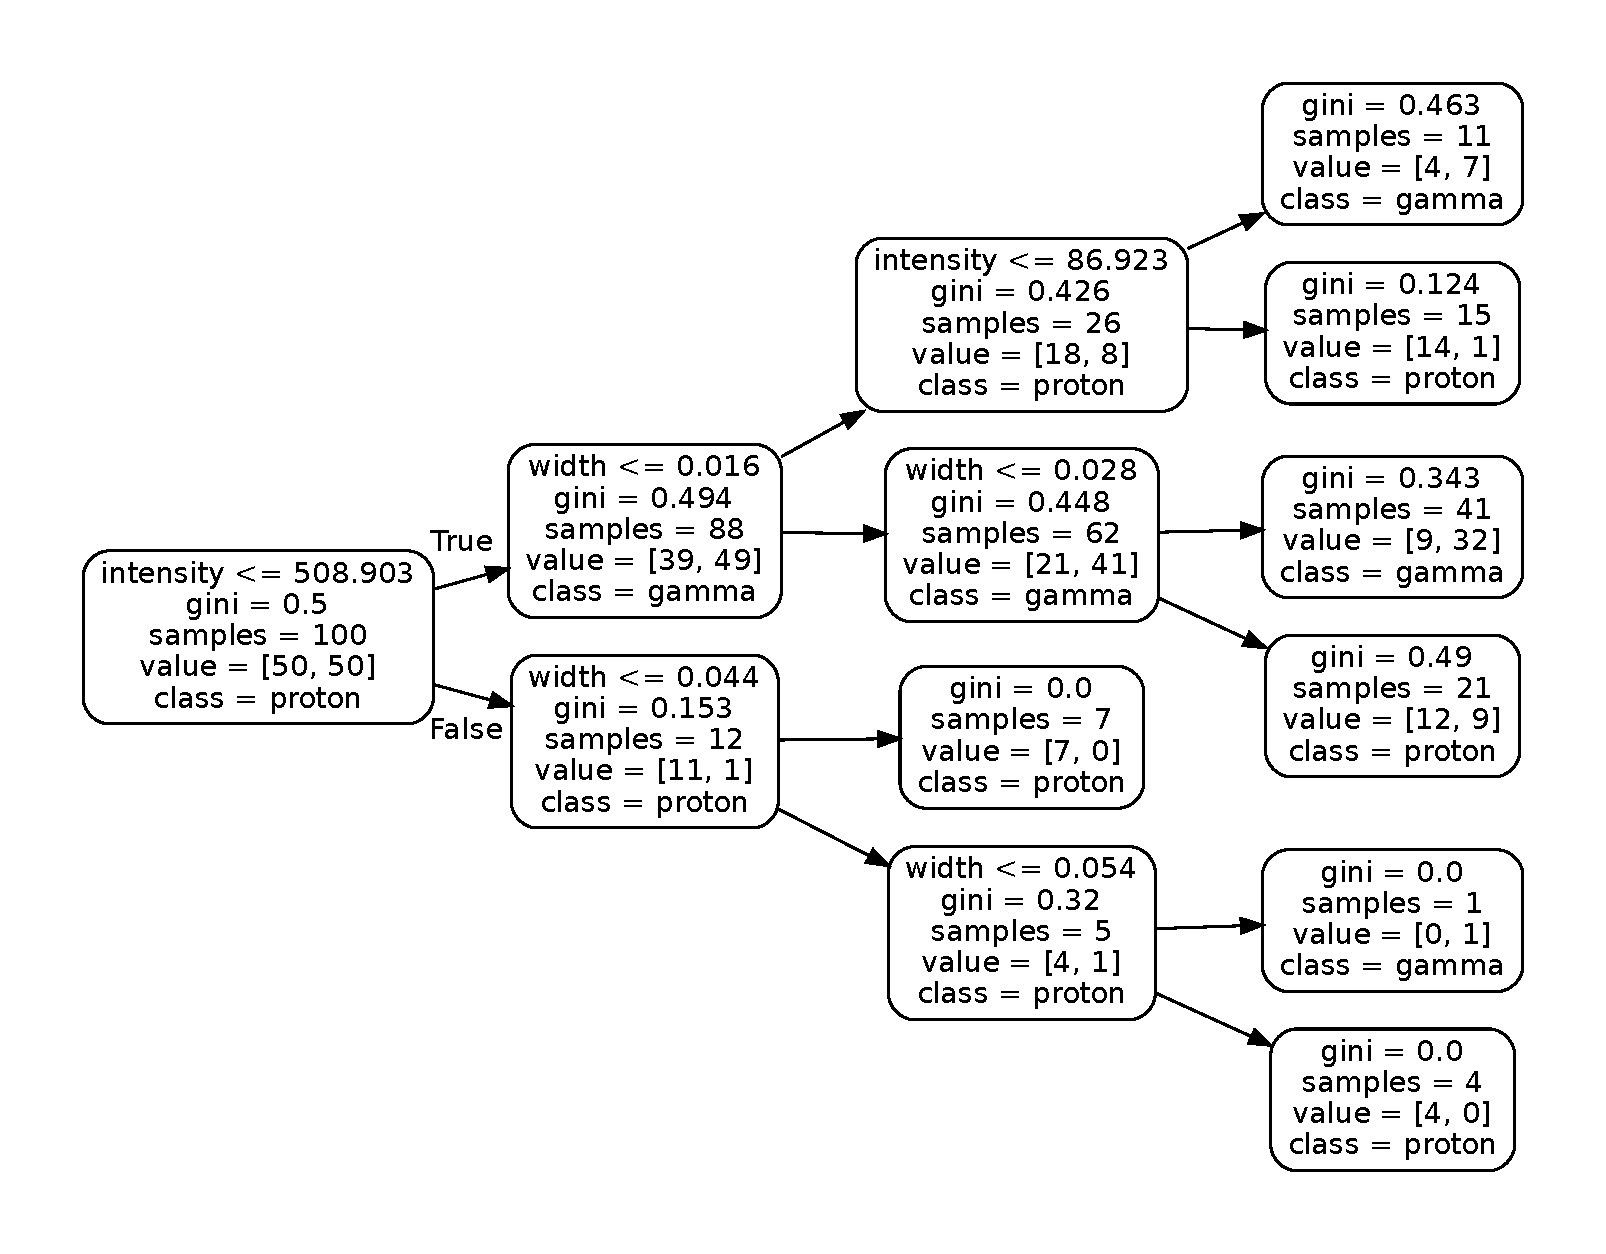
\includegraphics[width=0.7\textwidth]{Plots/decision_tree.pdf}
  \caption{Sample decision tree used to classify flowers in
  the iris dataset \cite{fisher1936use} \cite{sklearn}.}
  \label{fig:03_tree}
\end{figure}

Starting from the root node, a binary split is performed to
split up the data. For each split additional splits are performed
until a stopping criterion is reached.
How to choose the optimal split is defined as minimizing a
pre-defined measure. For classification tasks often used measures
are the above used gini coefficient (zitat) and the
cross-entropy (zitat).

indizes erklären!
\begin{equation}
  \text{Gini coefficient: } \\
  \text{Cross-entropy: }
  \label{eq:03_gini_ce}
\end{equation}

A stopping criterion can be defined as the measure reaching zero or
falling under a defined threshold.

For regression tasks the mean squared error or mean absolute error
are used and the same principles apply.
\begin{equation}
  \text{mse: } \\
  \text{mae: }
  \label{eq:03_mse_mae}
\end{equation}

To avoid overly complex trees, which would result in both high memory
consumption and potential overfitting on data, decision trees are often
limited to a certain depth, reducing the complexity of the model.
While decision trees have the benefit of providing
easily interpretable, low bias models there are some drawbacks to this
approach, namely \cite[hastie2017springer]:
\begin{itemize}
  \item{Instability, high variance}
  \item{Lack of Smoothness}
  \item{Difficulty in Capturing Additive Structure}.
\end{itemize}

Approaches to reducing these problems include
boosting \cite{freund1997decision} and Random Forests \cite{Breiman2001}.

\subsection{Random forests}
The main idea behind random forests is to use multiple, independent
decision trees to suppress the problems single trees have, while
keeping their advantages. For this to work, the individual trees need
need not to be correlated. Consequently the trees cannot all
be constructed the same way. Instead each tree performs splits
regarding a random subset of all available variables.
The Prediction of the random forest is then either the average of
the single predictions in case of a regression task or
the majority vote of the single predictions in case of classification.

Formel 15.1 aus hastie erklären

Random forests have become one of the standard algorithms
in our data analysis, because according to our
experience and \cite{hastie2017springer} they tend to
not overfit (as long as the individual trees have no or little bias)
and generally perform decent without a lot of manual tuning.


\section{mean estimation stuff, outlier resistance, unsupervised? clusters?}
warum robuste schätzer?
verwendete algorithmen
